I test di integrazione servono ad assicurare che le varie componenti funzionino correttamente quando messe in relazione.


\subsubsection{Test di integrazione previsti}

\begin{tabularx}{\textwidth}{cXc}
	
	\rowcolor{greySWEight}
	
	\rowcolor{greySWEight}
	\textcolor{white}{\textbf{Codice}} & 
	\textcolor{white}{\textbf{Descrizione}} &
	\textcolor{white}{\textbf{Stato}} \\

\textbf{TI001} & Verifica il corretto funzionamento tra UsersRepository e MongoDB & \textcolor{ForestGreen}{Superato} \\
\textbf{TI002} & Verifica il corretto funzionamento tra PhraseRepository e MongoDB & \textcolor{ForestGreen}{Superato} \\
\textbf{TI003} & Verifica il corretto funzionamento tra ExerciseRepository e MongoDB & \textcolor{ForestGreen}{Superato} \\
\textbf{TI004} & Verifica il corretto funzionamento tra UserService e UsersRepository & \textcolor{ForestGreen}{Superato} \\
\textbf{TI005} & Verifica il corretto funzionamento tra PhraseService e PhraseRepository & \textcolor{ForestGreen}{Superato} \\
\textbf{TI006} & Verifica il corretto funzionamento tra ExerciseService e ExerciseRepository & \textcolor{ForestGreen}{Superato} \\
\textbf{TI007} & Verifica il corretto funzionamento tra SolutionService e la connessione a FreeLing & \textcolor{ForestGreen}{Superato} \\
\textbf{TI008} & Verifica il corretto funzionamento tra Controller e UserService & \textcolor{ForestGreen}{Superato} \\
\textbf{TI009} & Verifica il corretto funzionamento tra Controller e SolutionService & \textcolor{ForestGreen}{Superato} \\
\textbf{TI010} & Verifica il corretto funzionamento tra Controller e ExerciseService & \textcolor{ForestGreen}{Superato} \\
	
	\rowcolor{white}
	\caption{Test di integrazione}
	\label{tab:tabellatestintegrazione}
\end{tabularx}

% \begin{figure}[H]
% 	\centering
% 	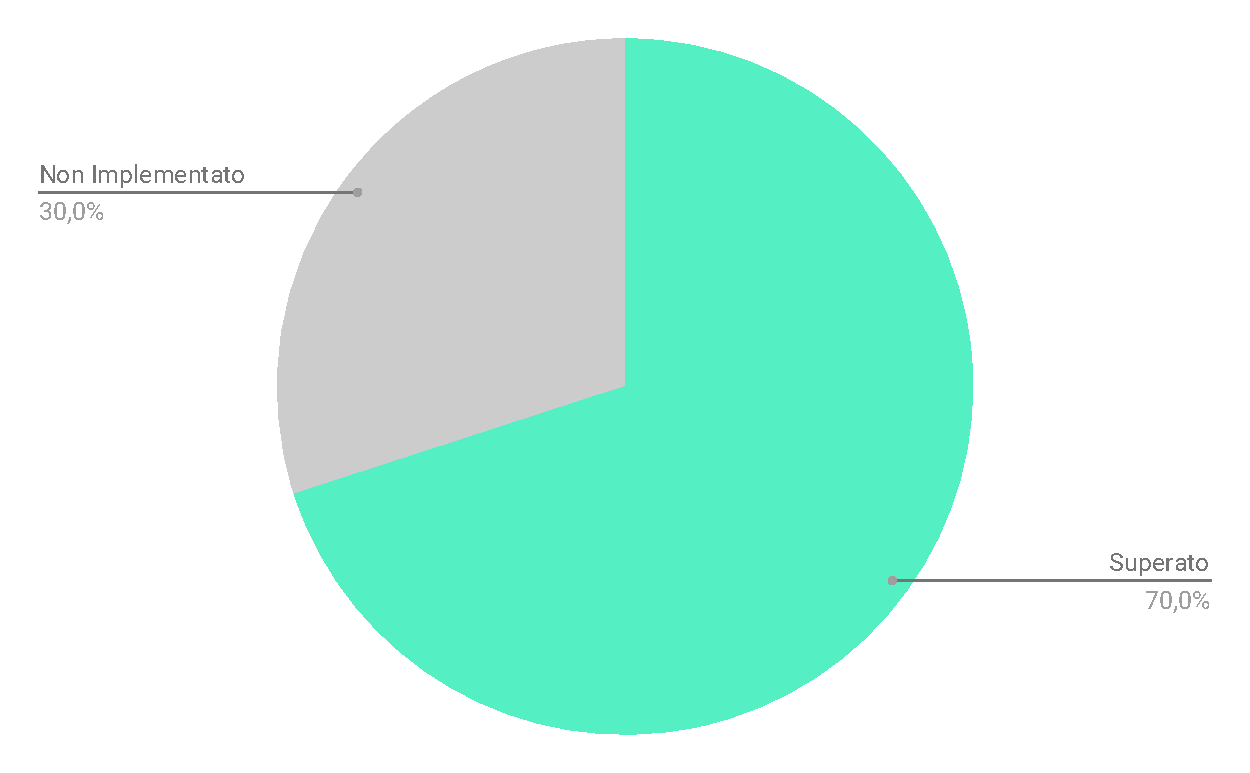
\includegraphics[width=0.7\linewidth]{sez/test/img/statoTestIntegrazione.pdf}
% 	\caption{Riepilogo stato test di integrazione}
% \end{figure}

\subsubsection{Tracciamento Test di integrazione - Componenti}

\begin{tabularx}{\textwidth}{cX}
	
	\rowcolor{greySWEight}
	
	\rowcolor{greySWEight}
	\textcolor{white}{\textbf{Test}} & 
	\textcolor{white}{\textbf{Componenti}} \\
	
	TI001 & colletta::repository::user::UsersRepository \\
	TI002 & colletta::repository::phrase::PhraseRepository \\
	TI003 & colletta::repository::exercise::ExerciseRepository \\
	TI004 & colletta::service::user::UserService \\
	TI005 & colletta::service::PhraseService \\
	TI006 & colletta::service::ExerciseService \\
	TI007 & colletta::service::SolutionService \\
	TI008 & colletta::controller::Controller \\
	TI009 & colletta::controller::Controller \\
	TI010 & colletta::controller::Controller \\
	
	\rowcolor{white}
	\caption{Tracciamento test di integrazione - componenti}
	\label{tab:tracciamentotestintegrazione}
\end{tabularx}
